\chapter{Introduction}

\section{Présentation de l'entreprise d'accueil}
Créée en 2003 par Laurent Py et Bruno LEGEARD, la société LEIROS est spécialisée dans le test logiciel. Elle est issue du projet Smart Testing\texttrademark ~au LIFC\footnote{Laboratoire d'informatique de Franche-Comté}. L'objectif premier de LEIROS a été d'industrialiser le projet Smart Testing\texttrademark.  LEIROS a ensuite changé de nom pour devenir SMARTESTING en juin 2008. En septembre 2008, Smartesting ouvre sa filiale à Bangalore, en Inde. SMARTESTING compte environ trente-cinq personnes dont onze dans le service R\&D{}\footnote{Recherche et développement}.

\begin{figure}[!ht]
\centering

\includegraphics[width=.55\textwidth]{Illustrations/temis.jpg}
\caption{Centre Temis à Besançon}
\label{figure:temis}
\end{figure}

\subparagraph*{}
Smartesting est implantée dans différents points stratégiques. En France,le siège social ainsi que le centre R\&D sont à Besançon dans les locaux de l'hôtel d'entreprises TEMIS Innovation(cf. figure\ref{figure:temis} p.\pageref{figure:temis}). Ainsi la R\&D reste proche géographiquement de l'université et de la recherche qui y a lieu. À Paris et à Amsterdam aux Pays-Bas se trouvent les agences où travaillent les commerciaux et les avant-vente. Smartesting s'est implantée à Bangalore, en Inde où elle compte réaliser la moitié de son chiffre d'affaires en 2010 grâce au boom de l'offshore où le marché du test logiciel est en pleine expansion.

\subparagraph*{}
Smartesting développe dans le secteur grandissant du test logiciel. Ce marché devrait atteindre 13 milliards de dollars en 2010 (selon une étude de Gartner). Le test logiciel, en particulier le test fonctionnel devient une phase clé du développement logiciel. Des besoins très stricts pour les milieux bancaires par exemple obligent ces entreprises à faire appel à des ingénieurs et des architectes de test afin de concevoir les tests logiciels qui permettront par exemple de garantir la stabilité, la non regression et le bon fonctionnement de gros projets. SMARTESTING propose Test Designer, une solution de génération automatique de référentiels de test à plusieurs niveaux.

\begin{figure}[!ht]
\centering
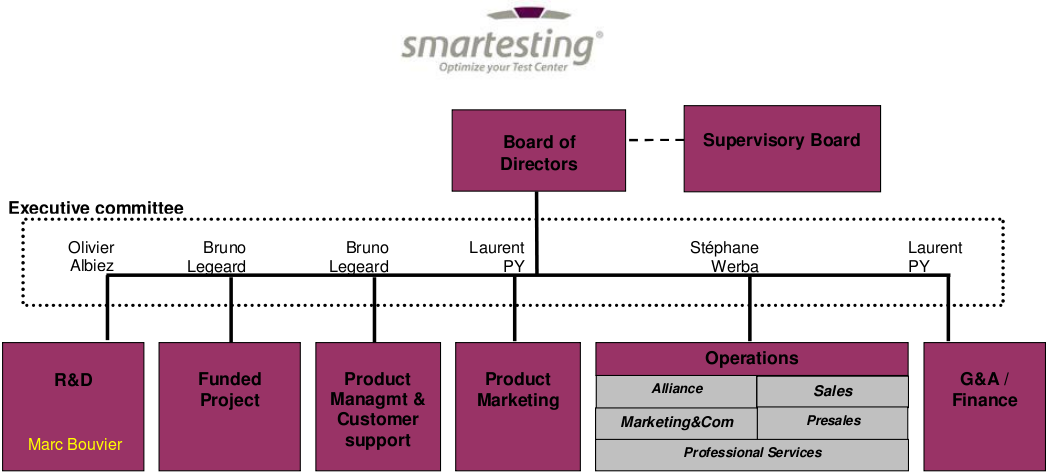
\includegraphics[width=\textwidth]{Illustrations/Organigramme_with_me.png}
\caption{Organigramme}
\label{figure:Organigramme de Smartesting}
\end{figure}

\subparagraph*{}
L'entreprise est organisée autour d'un directoire de trois personnes : Laurent PY, Bruno LEGEARD et Stéphane WERBA.Je travaille dans le service de R\&D{}\ de SMARTESTING.  L'équipe est composée de 11 ingénieurs dévelopeurs qui améliorent sans cesse le produit Test Designer ainsi que les connecteurs et les publishers y sont développés. L'équipe fonctionne autour de méthodes Agiles, en particulier eXtreme Programming. Ces sujets seront développés dans les sections qui vont suivre.

\pagebreak

\section{Test Designer}
La solution Test Designer permet de générer des référentiels de tests fonctionnels à partir de modèles UML pour le test/footnote{Model Based Testing}. Elle fait le lien entre la modélisation de tests et le management de tests.

%Figure 
\begin{figure}[!ht]
\centering
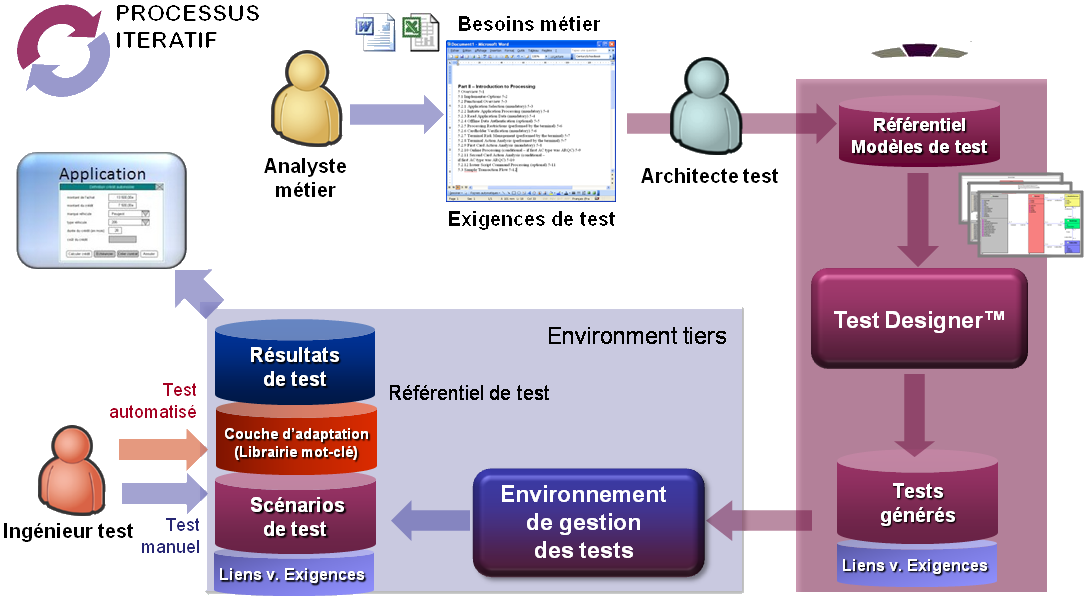
\includegraphics[width=\textwidth]{Illustrations/TheSolutionSmartesting.png}
\caption{La solution SMARTESTING}
\label{figure:La Solution SMARTESTING}
\end{figure}

\subparagraph*{}
La modélisation de tests se fait à l'aide de modeleurs UML basés sur Eclipse\footnote{Eclipse est une plateforme applicative sur laquelle peuvent se greffer des applications clientes sous forme de plugins(extensions)}. Les modeleurs supportés actuellement par Test Designer sont Borland Together 2008 et IBM Rational Software Modeler 7.0.5 \& 7.5. Il s'agit de modeleurs basés sur la plateforme Eclipse. Eclipse est une architecture de plugins qui communiquent les uns avec les autres pour former une application. C'est via ce mécanisme que Smartesting a développé deux plugins d'exportation de modèle pour les deux modeleurs précédemment cités.

\subparagraph*{}
Une fois le modèle de tests exporté il est utilisable par Test Designer pour générer automatiquement des référentiels de tests. Ces tests sont stockés dans un référentiel de test. Ces test pourront être publiés vers des evironnements tiers (HP Quality Center, tests JUnit, XML, Specifications pdf...).

\subparagraph*{}
Le processus de génération de tests de la solution Smartesting est un processus itératif. C'est à dire que si l'application déjà testée doit évoluée, la prise en compte des nouvelles fonctionnalités, ne générera pas un nouveau coût de génération des tests. 
Il suffit de modifier le modèle UML de spécifications via le modeleur, puis de générer les tests à nouveau (automatique). Ainsi les architectes de test gagnent un temps considérable à ne pas générer des test qui sont déja existants.

\subparagraph*{}
Traditionnellement la génération de tests est effectuée manuellement par un ingénieur de tests.

\section{Environnement de travail}
La première tâche qui m'a été confiée à mon arrivée fut d'installer mon poste de travail. Un ordinateur avec Ubuntu 8.10 m'a été confié et j'y ai installé IntelliJ Idea 8.0 (IDE\footnote{Environnement de développement intégré}), adapter quelques options de configuration au développement sur le projet Test Designer. Je me suis ensuite familiarisé pendant une semaine avec le code existant. La consigne était de ne demander d'aide de personne pendant une semaine. Au debut de la semaine qui suivit, je devais faire une compte rendu de ce que j'avais compris. Ce ``test'' permet en fait à l'équipe d'avoir un  marqueur sur la lisibilité du code source. Après cette phase d'apprentissage de l'existant, j'ai commencé à travailler sur des fonctionalités de Test Designer.

\subparagraph*{}
Le code source de Test Designer (le coeur de métier de SMARTESTING) est développée en JAVA avec un moteur de génération de tests qui s'appuie sur une approche prover (en c++). L'injection de dépendances est gérée par PICO. Une grande variété de bibliothèques sont utilisées telles que les google collections, JUnit, Mockito, JTidy, ou encore JYaml. Certaines ``boîtes à outils'' sont néanmoins développés en interne pour les besoins de la production. Les plugins dans les modeleurs utilisent l'architecture en plugin d'Eclipse pour s'y intégrer. En ce qui concerne les publishers, ils sont un fichier XML créé à partir du référentiel de tests. Ce fichier est ensuite exploité par le biais d'une API développée par l'équipe est distribuée aux clients lors de la livraison. Finalement l'API est aussi bien utilisée par les développeurs de l'équipe R\&D, les consultants de SMARTESTING que les clients finaux.